\chapter{Modelagem com redes neurais artificiais} \label{cha:model}

\section{Conceitos básicos} \label{sec:model-basic}

As redes neurais artificiais (ANN) são um tipo representativo dos modelos baseados na biologia, nos quais comportamentos e estruturas biológicas são reproduzidos através de funções e algoritmos, e, entre estes modelos, os algoritmos genéticos, de inteligência de enxame e as redes neurais artificiais se destacam pelo uso disseminado em diversas áreas da engenharia \cite{Darwish2018} \cite{Fan2020}.

A base das redes neurais artificiais é o perceptron, um modelo matemático do funcionamento dos neurônios presentes em nossos cérebros. Como passo inicial na analogia entre os perceptrons e os neurônios, os neurônios podem ser divididos, de modo muito simplificado, em três partes: os dendritos, o corpo e o axônio \cite{hall_tratado_2011}.

Os dendritos compõem os terminais de recepção do neurônio, no qual sinais provenientes de outros neurônios são recebidos e enviados para o corpo do neurônio. No corpo os sinais recebidos sofrem uma transformação não-linear e então são transmitidos para outros neurônios por meio do axônio.

De forma análoga, conforme a \autoref{fig:model-perceptron}, o perceptron é composto por uma região de recepção, da aplicação de uma função não-linear aos sinais de entradas e de uma etapa de transmissão para a camada seguinte de perceptrons. Através desta estrutura, o perceptron consegue separar qualquer região através de um plano n-dimensional \cite{haykin1999neural}.

\imagem{Modelo de perceptron com tangente hiperbólica}{
\resizebox{0.8\textwidth}{!}{
\begin{tikzpicture}[thick]
    \node[functions] (center) {$\tanh(.)$};
    \node[below of=center,font=\scriptsize,text width=4em] {\tiny Função de ativação};

    \node[right=2em of center] (right) {};
        \path[draw,->] (center) -- (right);
    
    \node[functions,left=2em of center] (left) {$\sum\limits_{i=1}^{N}(in_{i}w_{i})+b$};
        \path[draw,->] (left) -- (center);
    
    \node[weights,left=3em of left] (2) {$w_2$} -- (2) node[left of=2] (l2) {$in_2$};
        \path[draw,->] (l2) -- (2);
        \path[draw,->] (2) -- (left);
    \node[below of=2] (dots) {$\vdots$} -- (dots) node[left of=dots] (ldots) {$\vdots$};
    
    \node[weights,below of=dots] (n) {$w_N$} -- (n) node[left of=n] (ln) {$in_N$};
        \path[draw,->] (ln) -- (n);
        \path[draw,->] (n) -- (left);
    \node[weights,above of=2] (1) {$w_1$} -- (1) node[left of=1] (l1) {$in_1$};
        \path[draw,->] (l1) -- (1);
        \path[draw,->] (1) -- (left);
    
    \node[weights,above of=1] (0) {$b$} -- (0) node[left of=0] (l0) {$1$};
        \path[draw,->] (l0) -- (0);
        \path[draw,->] (0) -- (left);
    
    \node[below of=ln,font=\scriptsize] {\tiny Entradas};
    \node[below of=n,font=\scriptsize] {\tiny Pesos};
\end{tikzpicture}
}
\label{fig:model-perceptron}
}{O autor}{fig:model-perceptron}{}{Modelo de perceptron utilizando a função tangente hiperbólica como função de ativação, no qual $in_{i}$ são as entradas, $w_{i}$ os pesos e $b$ o viés.}

De forma mais detalhada, a \autoref{fig:model-perceptron} recebe um número $N$ de entradas e possui os pesos $w_i$ e o viés $b$ como coeficientes ajustáveis. As entradas são multiplicadas pelos pesos conforme os seus índices e então uma função não-linear, no caso deste trabalho a tangente hiperbólica, é aplicada ao resultado da soma das entradas ponderadas com o viés $b$. Esse processo também pode ser representado de forma matricial através da multiplicação de dois vetores, o que pode ser visto na equação \ref{eq:equacao_perceptron}, e então da aplicação da função não-linear.

\begin{align}
\begin{bmatrix}
1 \\ 
in_{1}\\ 
\vdots\\ 
in_{n}
\end{bmatrix}^{T}
\begin{bmatrix}
b\\ 
w_{1}\\ 
\vdots\\ 
w_{n}
\end{bmatrix}
=
\sum\limits_{i=1}^{n}
in_{i} \times w_{i} + b
\label{eq:equacao_perceptron}
\end{align}

Dentre as funções não-lineares usadas nas redes neurais artificiais as mais usadas são as funções sigmoides, ReLU e swish, em comum elas possuem características como serem monotônicas e uma região limitada de saída \cite{Szandaa2020}. A tangente hiperbólica faz parte das funções sigmoides e pode ser visualizada na \autoref{fig:tanh}, possuindo uma região de saída os valores entre -1 e 1 e sendo derivável em todos os seus pontos.

\imagem{Função tangente hiperbólica}{
\label{fig:tanh}
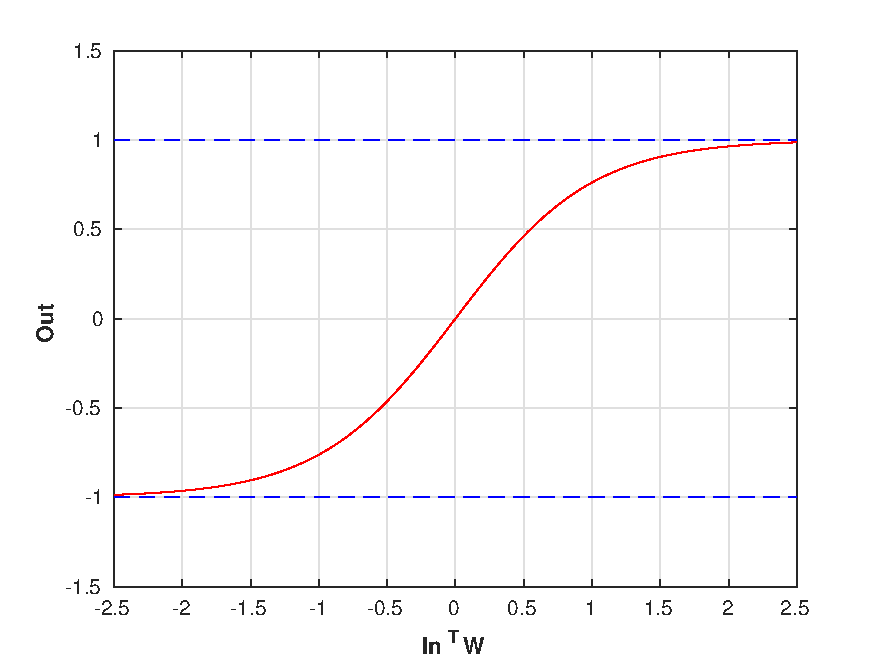
\includegraphics[width = 0.8\textwidth]{fig/sigmoide-eps-converted-to.pdf}
}{O autor}{fig:tanh}{}{Representação gráfica da função tangente hiperbólica para valores em torno de 0, mostrando o comportamento em formato de S.}

Enquanto os perceptrons conseguem separar uma região através de um hiperplano, eles não possuem individualmente a capacidade de reproduzir funções mais complexas \cite{haykin1999neural}. Para isso é necessário usar os perceptrons reunidos em camadas, no que é conhecido como perceptron de multicamada (MLP), no qual a camada de entrada recebe os dados, passa esses para as camadas ocultas de perceptrons e no final estes dados são passados para a camada de saída também composta por perceptrons e que adequa os dados para as dimensões e para o intervalo correto. O MLP possui em sua versão mais simples uma única camada oculta e é conhecido como perceptron de três camadas (TLP), que pode ser visto na figura (), que possui a capacidade de representar qualquer função através de um número arbitrário de coeficientes \cite{Hornik1991}.
\ExplSyntaxOn
\NewDocumentCommand{\storedata}{mm}{\tl_set:Nn#1{#2}}
\DeclareExpandableDocumentCommand{\getdata}{O{1}m}{\tl_item:Nn#2{#1}}
\ExplSyntaxOff
\def\layersep{2cm}
\storedata\mydata{{$in_{1}$}{$in_{2}$}{$in_{3}$}{$in_{4}$}{$in_{5}$}}

\imagem{Perceptron de três camadas}{
\label{fig:tlp}
\resizebox{0.8\textwidth}{!}{
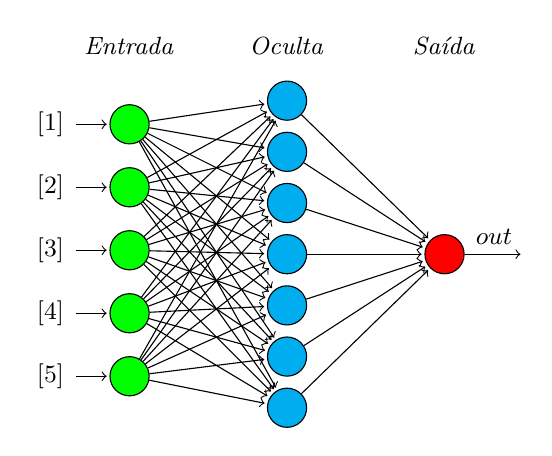
\begin{tikzpicture}[shorten >=1pt,->,draw=black, node distance=\layersep]
    \tikzstyle{every pin edge}=[<-,shorten <=1pt]
    \tikzstyle{neuron}=[circle,draw=black,minimum size=13pt,inner sep=5pt,font=\footnotesize]
    \tikzstyle{annot} = [text width=4em, text centered]

    % Draw the input layer nodes
    \foreach \name / \y in {1,...,5}
        \node[neuron, pin=left:{\small\getdata[\y]\mydata},fill=green] (I-\name) at (0,-0.8*\y) {};

    % Draw the hidden layer nodes
    \foreach \name / \y in {1,...,7}
        \path[yshift=0.15cm]
            node[neuron,fill=cyan] (H-\name) at (\layersep,-0.65*\y cm) {};

    % Draw the output layer node
    \node[neuron, right of=H-4,yshift=0.0cm,fill=red] (O) {};

    % Connect every node in the input layer with every node in the hidden layer.
    \foreach \source in {1,...,5}
        \foreach \dest in {1,...,7}
            \path (I-\source) edge 
            node[circle] {}(H-\dest);

    % Connect every node in the hidden layer with the output layer
    \foreach \source in {1,...,7}
        \path (H-\source) edge node[circle] {}(O);
        

     %Annotate the layers
    \node[annot,above of=H-1, node distance=0.70cm] (hl) {\small \textit{Oculta}};
    \node[annot,left of=hl] {\small \textit{Entrada}};
    \node[annot,right of=hl] {\small \textit{Saída}};
\node[coordinate,right of=O,node distance=1cm] (wabba){};
\draw [->] (O) -- node[above] {\small $out$}(wabba);
\end{tikzpicture}
}
}{O autor}{fig:tlp}{}{Diagrama de blocos de um \textit{perceptron} de três camadas com as entradas $in_i$ e a saída $out$ representadas.}

Assim como o funcionamento do perceptron pode ser individualmente representado através de operações matriciais, conforme a equação \autoref{eq:equacao_perceptron}, as operações de uma camada de perceptrons pode ser representada por meio da multiplicação do vetor de entradas pela matriz composta pelos coeficientes da camada, como pode ser visto na \autoref{eq:camada_oculta}, aonde N é o número de entradas e H o número de perceptrons na camada, e então pela aplicação da função de ativação para cada um dos membros do vetor de saída.

\begin{align}
\begin{bmatrix}
1 \\ 
in_{1}\\ 
\vdots\\ 
in_{N}
\end{bmatrix}^{T}
\begin{bmatrix}
b_{0}   & b_{1}   & \hdots & b_{H} \\ 
w_{1,0} & w_{1,1} & \hdots & w_{1,H} \\ 
\vdots  & \vdots  & \ddots & \vdots \\ 
w_{N,0} & w_{N,1} & \hdots & w_{N,H}
\end{bmatrix}
=
\begin{bmatrix}
\sum\limits_{i=1}^{n} in_{i} \times w_{i,0} + b_{0}\\ 
\sum\limits_{i=1}^{n} in_{i} \times w_{i,1} + b_{1}\\ 
\vdots\\ 
\sum\limits_{i=1}^{n} in_{i} \times w_{i,H} + b_{H}
\end{bmatrix}^{T}
\label{eq:camada_oculta}
\end{align}

\section{Treinamento e validação} \label{sec:model-trei}
Enquanto o teorema universal de aproximação informa que as o TLP pode aproximar qualquer função continua com os um conjunto arbitrário de coeficientes, esse número de coeficientes pode ser extremamente alto e a busca destes coeficientes não é coberta por esse teorema \cite{Goodfellow-et-al-2016}. Para se obter um conjunto de coeficientes que consiga generalizar uma função ainda é necessário que o processo de treinamento convirja para esse resultado através das consecutivas iterações, o mais conhecido entre os processos de treinamento para os coeficientes de uma rede neural artificial com múltiplas camadas é o processo conhecido como \textit{backpropagation}, que foi um dos primeiros algoritmos a conseguir ajustar de forma eficiente os coeficientes das camadas ocultas \cite{Goodfellow-et-al-2016} \cite{6302929}. Após o surgimento do \textit{backpropagation} outros algoritmos para o treinamento dos coeficientes foram encontrados \cite{Khidirova2020} \cite{Escalante2006}, o algoritmo utilizado nesse trabalho para o treinamento dos coeficientes foi o Levenberg–Marquardt \cite{Marquardt1963}.

Independente do algoritmo de treinamento utilizado, o processo de treinamento supervisionado de uma rede neural artificial requer um conjunto de amostras de entrada e de saída, sendo que no caso do treinamento de sistemas com memória as amostras devem estar organizadas temporalmente. O processo de treinamento realiza um ajuste iterativo dos coeficientes, normalmente utilizando as informações do gradiente das respostas, em busca de valores que minimizem uma função de perda que implique na aproximação do modelo ao sistema utilizado. De modo geral, os valores iniciais dos coeficientes podem ser escolhidos de maneira aleatória.

Como o modelo é treinado com um número finito de dados, é necessária a validação do mesmo com um segundo conjunto de entradas e saídas. A validação é essencial para garantir que não ocorram efeitos como o overfitting, no qual o modelo se ajusta perfeitamente a um conjunto específico de dados, mas não é capaz de reproduzir de maneira consistente o comportamento fora deste escopo \cite{haykin1999neural}. O conjunto de dados da validação é aplicado de forma a extrair os resultados da função de perda, a mesma função utilizada no treinamento.

Outras métricas podem ser usadas adicionalmente para se avaliar o comportamento do modelo durante e após o treinamento, neste trabalho a principal métrica utilizada foi o erro quadrático médio normalizado (NMSE), expresso através da \autoref{eq:nmse}.

\begin{align}
NMSE = 10\log_{10}
\left(
\frac
{\sum\limits_{i=1}^{N}
\abs{O_{i}-\widehat{O}_{i}}^{2}}
{\sum\limits_{i=1}^{N}
\abs{O_{i}}^2}
\right)
\label{eq:nmse}
\end{align}

\section{Topologia utilizada} \label{sec:model-topo}
Uma das principais características dos sinais dos amplificadores de potência é a sua representação por meio da utilização de números complexos, em razão disso o modelo utilizado deve possuir uma arquitetura capaz de representar os valores em suas componentes de amplitude e fase ou a partir da representação retangular. Em ambos os casos dois valores reais são necessários para representar cada amostra de entrada ou de saída do sinal.

Nesse trabalho a arquitetura utilizada, proposta em \cite{chipansky_freire_modfied_2015}, utiliza dois TLP para a extração da parte real e imaginária conforme a \autoref{fig:model-topo}. O modelo recebe o valor absoluto $a_x$ e a fase $\theta_x$ do sinal de entrada, assim como os valores passados numa profundidade de memória $M$. Os $M+1$ valores absolutos são passados diretamente como entrada para as duas redes neurais, enquanto as $M+1$ fases são usadas para determinar $M$ mudanças de fases conforme a equação \autoref{eq:diff_fase}, na qual $n$ é o número da amostra e $m$ assume os valores entre $0$ e $M$. As diferenças de fases são passadas como entradas para as funções senos e cossenos, para então estes valores tomarem seu lugar como entradas para os dois TLP.
%\criarsimbolo{$\angle$}{Fase de um número complexo}\label{item:fase}

\begin{align}
\Delta\theta_x(n,m) = \theta_x(n-m+1)-\theta_x(n-m)
\label{eq:diff_fase}
\end{align}

\imagemS{Topologia utilizada}{
\begin{adjustbox}{scale=2.0,center}
%\resizebox{0.8\textwidth}{!}{
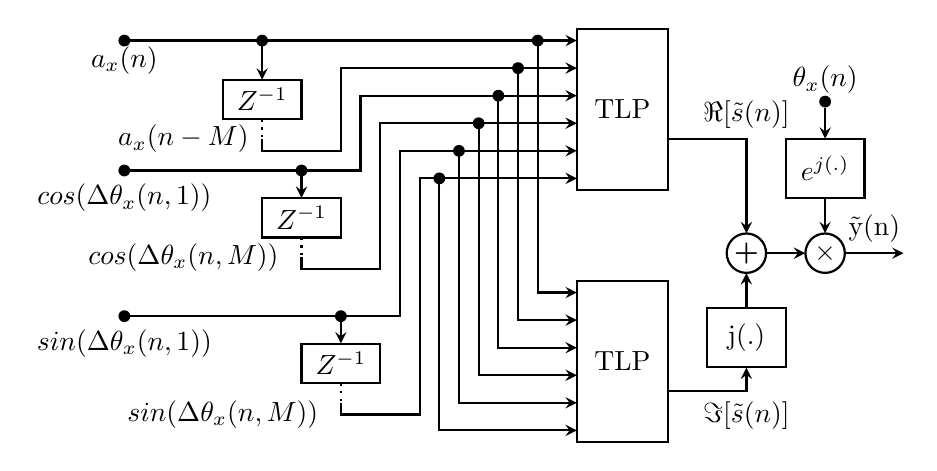
\begin{tikzpicture}[shorten <=0.1pt,shorten >=0.1pt,>=stealth,thick,->]

\draw  (-2,3.9) rectangle node {TLP} (-0.85,5.95);
\draw  (-2,7.1) rectangle node {TLP} (-0.85,9.15);

\draw  [thick,->,>=stealth] (-7.75,9) -- (-2,9);

\node [circle,minimum size=1.5mm,inner sep=0pt,outer sep=0pt,fill=black] at (-2.5,9) {};
\node [circle,minimum size=1.5mm,inner sep=0pt,outer sep=0pt,fill=black] at (-3,8.3) {};
\node[circle,minimum size=1.5mm,inner sep=0pt,outer sep=0pt,fill=black] at (-3.25,7.95) {};
\node[circle,minimum size=1.5mm,inner sep=0pt,outer sep=0pt,fill=black] at (-3.5,7.6) {};
\node[circle,minimum size=1.5mm,inner sep=0pt,outer sep=0pt,fill=black] at (-3.75,7.25) {};
\node  [circle,minimum size=1.5mm,inner sep=0pt,outer sep=0pt,fill=black] at (-2.75,8.65) {};
\node[circle,minimum size=1.5mm,inner sep=0pt,outer sep=0pt,fill=black] at (-6,9) {};
\node [circle,minimum size=1.5mm,inner sep=0pt,outer sep=0pt,fill=black] at (-5.5,7.35) {};
\node[circle,minimum size=1.5mm,inner sep=0pt,outer sep=0pt,fill=black] at (-5,5.5) {};

\draw (-2.5,9) -- (-2.5,5.8) -- (-2,5.8);

\draw (-6,7.75) -- (-6,7.6) -- (-5,7.6) -- (-5,8.65) -- (-2,8.65);

\draw (-7.75,7.35) -- (-4.75,7.35) -- (-4.75,8.3) -- (-2,8.3);

\draw (-2.75,8.65) -- (-2.75,5.45) -- (-2,5.45);
\draw (-3,8.3) -- (-3,5.1) -- (-2,5.1);
\draw (-5.5,6.25) -- (-5.5,6.1) -- (-4.5,6.1) -- (-4.5,7.95) node (v3) {} -- (-2,7.95);

\draw (-3.25,7.95) -- (-3.25,4.75) -- (-2,4.75);
\draw (-3.5,7.6) -- (-3.5,4.4) -- (-2,4.4);
\draw (-3.75,7.25) -- (-3.75,4.05) -- (-2,4.05);

\draw (-7.75,5.5) -- (-4.25,5.5) -- (-4.25,7.6) -- (-2,7.6);
\draw (-5,4.4) -- (-5,4.25) -- (-4,4.25) -- (-4,7.25) -- (-2,7.25);
\draw (-0.85,7.75) -- (0.15,7.75) node[above]{$\Re[\tilde{s}(n)]$} -- (0.15,6.55);
\draw (-0.85,4.55) --  (0.15,4.55) node[below] {$\Im[\tilde{s}(n)]$}-- (0.15,4.85);

\draw  (0.15,6.3) ellipse (0.25 and 0.25);
\draw (0.4,6.3) -- (0.9,6.3);
\draw (1.15,7) -- (1.15,6.55);
\draw  (1.15,6.3) ellipse (0.25 and 0.25);
\draw (1.4,6.3) -- node[above] {\~y(n)} (2.15,6.3);
\draw  (-0.35,5.6) rectangle node{j(.)} (0.65,4.85);
\draw (0.15,5.6) -- (0.15,6.05);
\draw  (0.65,7.75) rectangle node {$e^{j(.)}$} (1.65,7);
\draw (1.15,8.15) -- (1.15,7.75);
\draw  (-5.5,5.15) rectangle node {$Z^{-1}$} (-4.5,4.65);
\draw  (-6,7) rectangle node {$Z^{-1}$} (-5,6.5);
\draw  (-6.5,8.5) rectangle node {$Z^{-1}$} (-5.5,8);

\draw (-5.5,7.35) -- (-5.5,7);
\draw (-6,9) -- (-6,8.5);
\draw (-5,5.5) -- (-5,5.15);

\draw[dotted,-] (-6,8) -- (-6,7.75);
\draw[dotted,-] (-5.5,6.5) -- (-5.5,6.25);
\draw[dotted,-] (-5,4.65) -- (-5,4.4);

\node at (-7.75,8.75) {$a_{x}(n)$};
\node at (-7.75,7) {$cos(\Delta\theta_x(n,1))$};
\node at (-7.75,5.15) {$sin(\Delta\theta_x(n,1))$};

\node at (-7,7.75) {$a_{x}(n-M)$};
\node at (-7,6.25) {$cos(\Delta\theta_x(n,M))$};
\node at (-6.5,4.25) {$sin(\Delta\theta_x(n,M))$};

\node at (0.15,6.3) {\textbf{+}};
\node at (1.15,6.3) {$\times$};

\node [circle,minimum size=1.5mm,inner sep=0pt,outer sep=0pt,fill=black] at (-7.75,9) {};
\node [circle,minimum size=1.5mm,inner sep=0pt,outer sep=0pt,fill=black] at (-7.75,7.35) {};
\node [circle,minimum size=1.5mm,inner sep=0pt,outer sep=0pt,fill=black] at (-7.75,5.5) {};
\node [circle,minimum size=1.5mm,inner sep=0pt,outer sep=0pt,fill=black,above] at (1.15,8.15) {};
\node at (1.15,8.5) {$\theta_{x}(n)$};
\end{tikzpicture}
\end{adjustbox}
\label{fig:model-topo}
}
{O autor}{fig:model-topo}{}{Diagrama de blocos da topologia utilizada para a modelagem do PA e suas inversas.}
